\documentclass[../../dd.tex]{subfiles}

% Document
\begin{document}
\chapter{Architectural Design}
    \section{Overview}
    From an external point of view, users using their smartphones exploit the different
    services offered by \textit{Baddy} that are different for clients and caregivers.
    The application to be developed is based on one application component (application logic) which manages the interactions
    between different components of the system.
    Application logic is present both in the mobile view and in the back-end logic.
    In the mobile view there is the management of the GUI and the connection with other useful components
    present in the smartphone like GPS and camera; in the back-end logic instead there is the most of the logic and also the interfaces to external services:
    Database provider, Storage provider and Push notification provider.
    
    
     \begin{figure}[H]
        \centering
        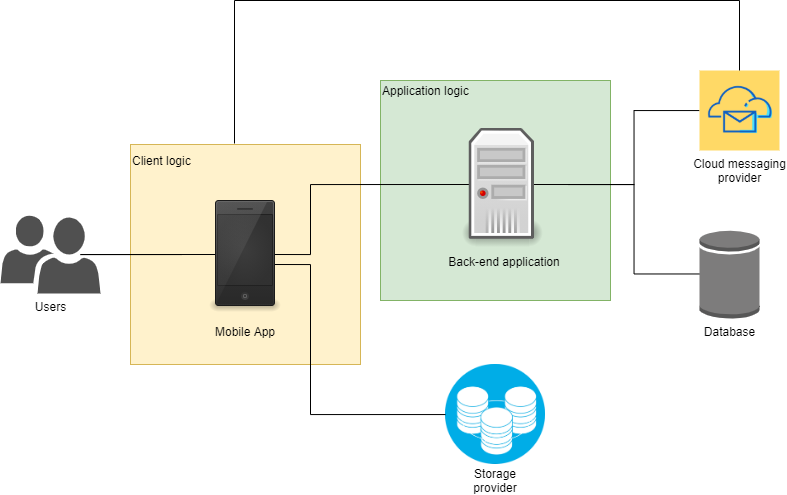
\includegraphics[scale=0.5]{assets/overview.png}\\[1.6 cm]
        \caption[\textit{Deployment} Diagram]{Overview of the application components}
    \end{figure}
    %todo add photo
    \section{Component View}
    %todo add photo
    In this section the system will be described in terms of its components: their
    functionalities will be discussed and detailed. Moreover, interfaces among components and among external systems will be shown.
    
    
    \subsection{Database}
    The application database is managed using a Non-Relational DBMS.
    It allows the reading of data, ensuring to the users the possibility to log in and check the stored data.
    It is also used for data manipulation (insertion, modification and deletion).
    The database offers to the Application Server an interface that it can use
    to interact with it.
    Particular attention must be paid to the encryption of passwords used to the user access to the system.

    \subsection{Application Server}
    The main feature of the Application Server is to define rules and work-flows
    of all the functionalities defined by the RestfulAPI.
    The Application Server must have interfaces to communicate with the Mobile
    Application and also with the DBMS; the communication must be done using
    the HTTPS protocol.
    In the brief introduction below, logic modules and their descriptions are
    presented, while all the connections among them can be seen in the Global
    Component View.
    \begin{itemize}
        \item \textbf{authController:} This module handles the authentication and authorization process.
        It generates authorization tokens and checks their validity.
        \item \textbf{errorController:} It manages all the routes that are not available and all the bad formatted requests.
        \item \textbf{handlerFactory:} General service that implements all CRUD operations.
        \item \textbf{reviewsController:} It manages all the newly created reviews with all the rankings.
        \item \textbf{usersController:} It manages users operations, like insertion of a new offer and updating profile.
    \end{itemize}

    \subsection{Mobile Application}
    The mobile application communicates with the Application Server
    through RestfulAPIs that are defined in order to describe the interactions
    between the two layers and that must be independent of the two implementations. More details about the implementation will be provided in the following sections.
    
    \newpage
    \section{Deployment View}
    In this section a deployment diagram details the execution architecture of the system, including nodes such as hardware or software execution environments, and the middleware connecting them.
    
    \begin{figure}[H]
        \centering
        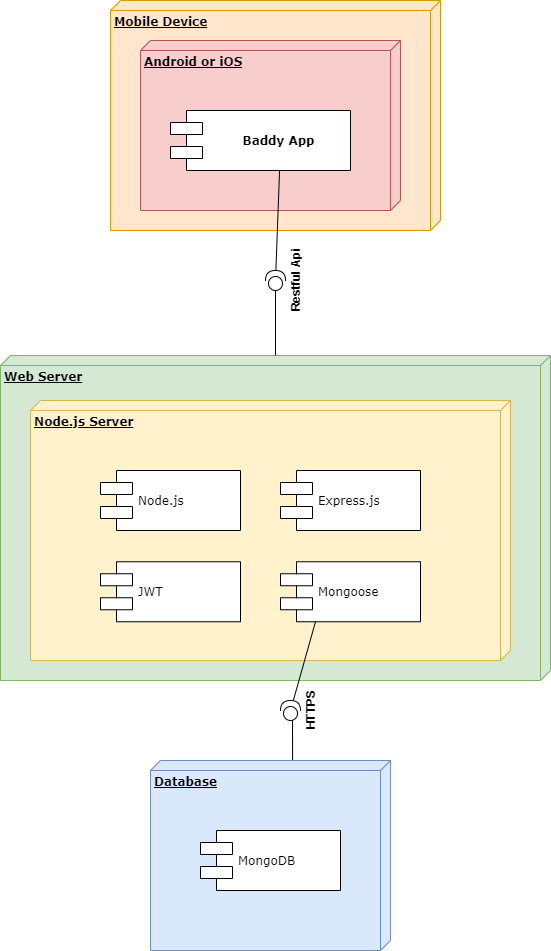
\includegraphics[scale=0.5]{assets/deployment2.png}\\[1.6 cm]
        \caption[\textit{Deployment} Diagram]{ Deployment diagram}
    \end{figure}
    
    
    \subsection{SEQUENCE TODO}
    
    
    \subsection{Selected architectural styles and Patterns}




\end{document}
